\section{Zustandsreglerentwurf} \label{sec:Zustandsreglerentwurf}

\subsection{Einfache Zustandsrückführung} \label{sec:Einfach}

Auf Basis der Reglerstruktur aus \autoref{fig:Bild7} folgt das notwendige Reglergesetz zu:\\
\newline

Reglergesetz:

\begin{align}
    \underline{u}(t) &= -\underline{k}\cdot\underline{x}(t)
    \label{eq:Gleichung19}
\end{align}

\begin{figure}[H]
   \centering
   \fbox{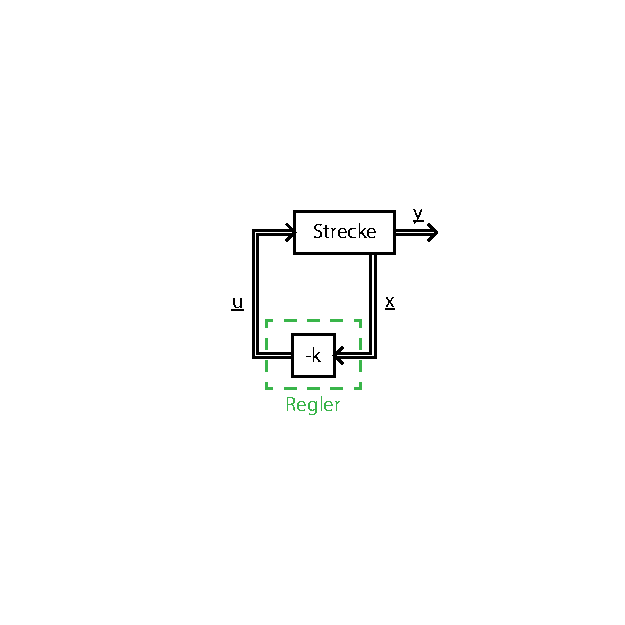
\includegraphics[width=0.3\textwidth]{Bilder/5_zustandsreglerentwurf/Reglerstruktur_einfache_Zustandsrueckfuehrung.pdf}}
   \caption[Reglerstruktur der einfache Zustandsrückführung]{Reglerstruktur der einfachen Zustandsrückführung}
   \label{fig:Bild7}
\end{figure}

Die Berechnung der k-Faktoren wird mittels linearen Matrixungleichungen mithilfe von Matlab gelöst. Hierbei wird die exponentielle Stabilität mit der Decay-Rate $\alpha$ berücksichtigt.\\
\newline

Matrixungleichung:

\begin{align}
        \begin{split}
        \underline{X}\cdot \underline{A}^'+\underline{A}\cdot\underline{X} -\underline{M}^'\cdot\underline{B}^' - \underline{B}\cdot \underline{M} +2\cdot\alpha\cdot \underline{X} < 0 \\
    \underline{X} > 0
    \end{split}
    \label{eq:Gleichung20}
\end{align}

mit:

\begin{align*}
    \underline{X} &= \underline{x} \quad X\in\mathbb{R}^{(2x1)}\\
    \underline{M} &= \underline{k}\cdot\underline{X} \quad M\in\mathbb{R}^{(1x2)}
\end{align*}

Die k-Faktoren folgen aus: $k = M\cdot X^{-1}$. Die Decay-Rate wird mit 0.5 vorgesehen.\\
\newline

k-Faktoren:

\begin{align}
    k &= 
    \begin{bmatrix}
        0.7105\cdot 10^{-3} & 0.0105\cdot 10^{-3}
    \end{bmatrix}
    \label{eq:Gleichung21}
\end{align}

Die Lage der Reglerpolstellen im Vergleich zu den Polstellen der Systemmatrix A sind in \autoref{fig:Bild8} visualisiert. Die Berechnung der Reglerpolstellen ist folgendermaßen definiert:\\
\newline

Berechnung der Reglerpolstellen:

\begin{align*}
    sP &= eig\left(\underline{A}-\underline{B}\cdot\underline{k}\right)
\end{align*}

\begin{figure}[H]
   \centering
   \fbox{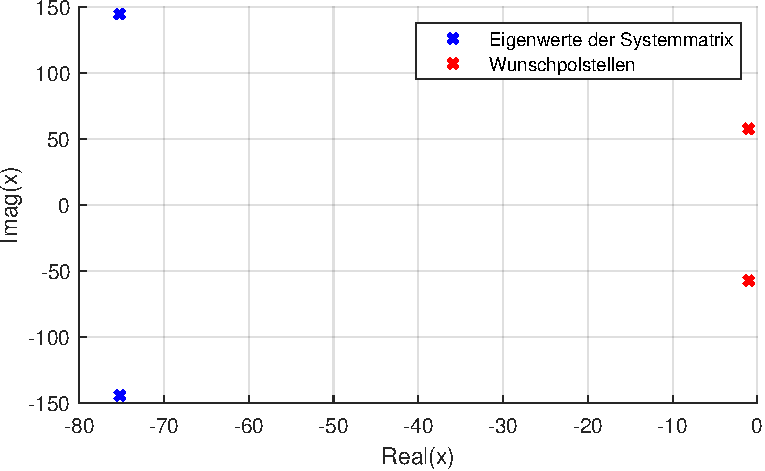
\includegraphics[width=0.75\textwidth]{Bilder/5_zustandsreglerentwurf/Polstellen_einfache_Rueckfuehrung.pdf}}
   \caption[Polstellenlage der einfache Zustandsrückführung]{Polstellenlage der einfachen Zustandsrückführung im Vergleich zur Systemmatrix}
   \label{fig:Bild8}
\end{figure}

\clearpage

\subsection{Referenzwertvorsteuerung} \label{sec:Referenzwertvorsteuerung}

Die Reglerstruktur wird erweitert, sodass nun eine Referenzspannung vorgegeben wird. Diese wird mit einem Vorfilter F verrechnet (\autoref{fig:Bild9}).

\begin{figure}[H]
   \centering
   \fbox{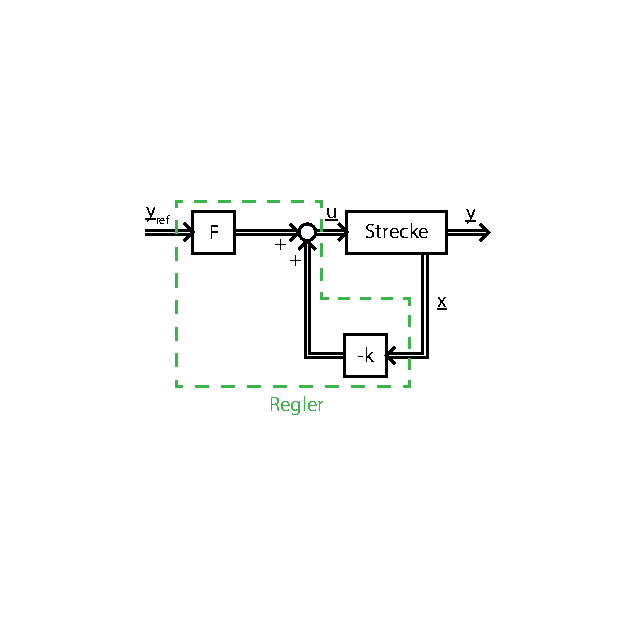
\includegraphics[width=0.5\textwidth]{Bilder/5_zustandsreglerentwurf/Reglerstruktur_Vorsteuerung.pdf}}
   \caption[Reglerstruktur der Referenzwertvorsteuerung]{Reglerstruktur der Referenzwertvorsteuerung}
   \label{fig:Bild9}
\end{figure}

Das Reglergesetz resultiert zu:\\
\newline

Reglergesetz:

\begin{align}
    \underline{u}(t) &= -\underline{k}\cdot\underline{x}(t)+\underline{F}\cdot\underline{y}_{\mathrm{ref}(t)}
    \label{eq:Gleichung22}
\end{align}

Die Berechnung der k-Faktoren erfolgt analog zum \autoref{sec:Einfach} mit einer Decay-Rate $\alpha = 0.5$.\\
\newline

k-Faktoren:

\begin{align}
    k &= 
    \begin{bmatrix}
        -0.7105\cdot 10^{-3} & 0.0105\cdot 10^{-3}
    \end{bmatrix}
    \label{eq:Gleichung23}
\end{align}

Die Reglerpolstellen und die Eigenwerte der Systemmatrix werden in \autoref{fig:Bild10} dargelegt.

\begin{figure}[H]
   \centering
   \fbox{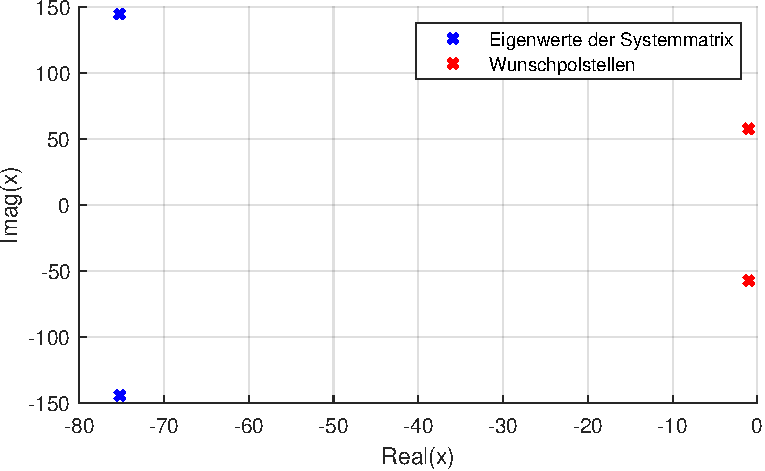
\includegraphics[width=0.75\textwidth]{Bilder/5_zustandsreglerentwurf/Polstellen_Referenzwertvorsteuerung.pdf}}
   \caption[Polstellenlage der Referenzwertvorsteuerung]{Polstellenlage der Referenzwertvorsteuerung im Vergleich zur Systemmatrix}
   \label{fig:Bild10}
\end{figure}

Die Berechnung des Vorfilters F wird auf Grundlage der \autoref{eq:Gleichung24} durchgeführt.

\begin{align}
    \underline{F} &= \left(C_{\mathrm{Vor}}\cdot\left(-\underline{A}+\underline{B}\cdot\underline{k}\right)^{-1}\cdot\underline{B}\right)^{-1}
    \label{eq:Gleichung24}
\end{align}

mit:

\begin{align*}
    C_{\mathrm{Vor}} &= 
    \begin{bmatrix}
        1 & 0
    \end{bmatrix}
\end{align*}

Die Berechnung des Vorfilters ergibt: $F = -1.0193\cdot 10^{-4}$.

\clearpage

\subsection{I-Regelung} \label{sec:Iregler}

Das anzuwendene Reglergesetz folgt aus der Reglerstruktur in \autoref{fig:Bild11}.

\begin{figure}[H]
   \centering
   \fbox{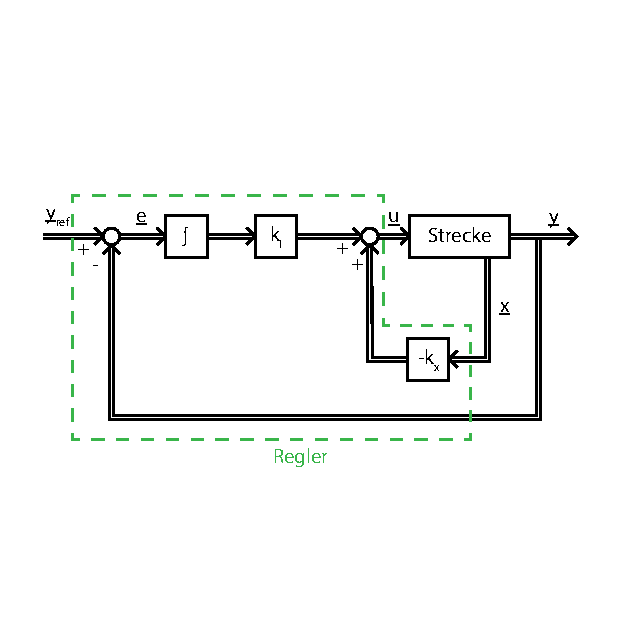
\includegraphics[width=0.7\textwidth]{Bilder/5_zustandsreglerentwurf/Reglerstruktur_I_Regelung.pdf}}
   \caption[Reglerstruktur der I-Regelung]{Reglerstruktur der Regelung mit Integrationsglied}
   \label{fig:Bild11}
\end{figure}

Reglergesetz:

\begin{align}
    \underline{u} &= \underline{k}_{\mathrm{I}}\cdot\int_{0}^t(\underline{y}_{\mathrm{ref}}-\underline{y})d\tau-\underline{k}_{\mathrm{x}}\cdot\underline{x}
    \label{eq:Gleichung25}
\end{align}

Zur Vereinfachung wird nachfolgende Definition eingesetzt.\\
\newline

Definition:

\begin{align*}
    \underline{x}_{\mathrm{I}}& :=\int_{0}^t(\underline{y}_{\mathrm{ref}}-\underline{y})d\tau
\end{align*}

Einsetzen der Definition:

\begin{align}
    \underline{u} &= \underline{k}_{\mathrm{I}}\cdot\underline{x}_{\mathrm{I}}-\underline{k}_{\mathrm{x}}\cdot\underline{x} \\ \nonumber \\
    \underline{u} &= -
    \begin{bmatrix}
        \underline{k}_{\mathrm{x}} & -\underline{k}_{\mathrm{I}}
    \end{bmatrix}
    \cdot
    \begin{bmatrix}
        \underline{x} \\
        \underline{x}_{\mathrm{I}}
    \end{bmatrix}
    \nonumber
\end{align}

mit:

\begin{align}
    \underline{\tilde{k}} &= 
    \begin{bmatrix}
    \underline{k}_{\mathrm{x}} & -\underline{k}_{\mathrm{I}}
    \end{bmatrix}
    \label{eq:Gleichung27}
\end{align}

Zur Berechnung der k-Faktoren wird ein erweitertes Zustandsraummodell eingeführt.\\
\newline

Erweitertes Zustandsraummodell:

\begin{align}
    \underline{\dot{\tilde{x}}} &= 
    \begin{bmatrix}
        \underline{A} & \underline{0} \\
        -\underline{C} & \underline{0}
    \end{bmatrix} \cdot \underline{\tilde{x}} +
    \begin{bmatrix}
        \underline{B} \\
        \underline{0}
    \end{bmatrix} \cdot\underline{u} +
    \begin{bmatrix}
        \underline{0} \\
        \underline{I}
    \end{bmatrix} \cdot\underline{y}_{ref}
    \label{eq:Gleichung28}
\end{align}

mit:

\begin{align*}
    \underline{\tilde{A}} &= 
    \begin{bmatrix}
        \underline{A} & \underline{0} \\
        -\underline{C} & \underline{0}
    \end{bmatrix} \quad ; \underline{\tilde{A}}\in\mathbb{R}^{(n+p)x(n+p)}\\
    \underline{\tilde{B}} &= 
    \begin{bmatrix}
        \underline{B} \\
        \underline{0}
    \end{bmatrix}\qquad ; \underline{\tilde{B}}\in\mathbb{R}^{(n+p)x(m)}\\
    \underline{\tilde{B}}_{\mathrm{y}} &= 
    \begin{bmatrix}
        \underline{0} \\
        \underline{I}
    \end{bmatrix}\qquad  ;\underline{\tilde{B}}_{\mathrm{y}}\in\mathbb{R}^{(n+p)x(p)}
\end{align*}

Die Matrix C wird wie in \autoref{sec:Referenzwertvorsteuerung} definiert. Somit folgen die Matrizen $\tilde{A}$ und $\tilde{B}$ nach der Definition zu:

\begin{align*}
    \tilde{A} &=
    \begin{bmatrix}
        -150.4187 & -54.5419 & 0 \\
        486.5101 & 0 & 0 \\
        -1 & 0 & 0
    \end{bmatrix} \\
    \tilde{B} &=
    \begin{bmatrix}
        -2.1763\cdot 10^5 \\
        5.9499\cdot 10^5 \\
        0
    \end{bmatrix}
\end{align*}

Die anschließende Berechnung der notwendigen k-Faktoren erfolgt analog zu \autoref{sec:Referenzwertvorsteuerung} mit den Tilde-Matrizen und $X\in\mathbb{R}^{(3x1)}$ und $M\in\mathbb{R}^{(1x3)}$. Die Decay-Rate wird auf 0.5 festgelegt. Zur Veranschaulichung der Polstellenlagen dient \autoref{fig:Bild12}.\\
\newline

k-Faktoren:

\begin{align}
    k &=
    \begin{bmatrix}
        0.6007\cdot 10^{-3} & -0.0258\cdot 10^{-3} & 0.2301\cdot 10^{-3}
    \end{bmatrix}
\end{align}

\begin{figure}[H]
   \centering
   \fbox{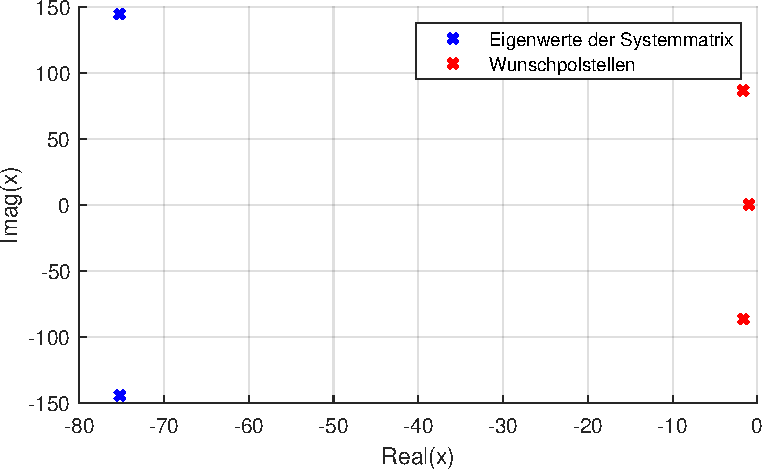
\includegraphics[width=0.75\textwidth]{Bilder/5_zustandsreglerentwurf/Polstellen_I_Regelung.pdf}}
   \caption[Polstellenlage der Referenzwertvorsteuerung mit I-Anteil]{Polstellenlage der Referenzwertvorsteuerung mit I-Anteil im Vergleich zur Systemmatrix}
   \label{fig:Bild12}
\end{figure}

